\chapter{Diseño}


\section{Fuentes de datos}
Al ser este un sistema \acrshort{RI} el diseño ha de girar en torno a los datos, por ello comencé explorando diversas alternativas para utilizar como fuente de datos. 

Como punto inicial para la extracción de los datos de los autores de la \acrshort{ETSIIT} partí del Ranking UGRinvestiga \cite{Ranking_UGRInvestiga}. En este se lista a todos los autores de la escuela junto con sus citas e índice h total y los últimos 5 años.

Sin embargo no hay modo de obtener datos de los artículos concretos por lo que barajé múltiples bases de datos bibliográficas, además de las ya comentadas en la sección \nameref{subsec:sistemasRI} también exploré \href{https://www.researchgate.net/}{Research Gate}.

Los resultados de mi análisis fueron los siguientes: 
\label{ls:dataSourceAnalisis}
\begin{itemize}
	
	\item Google Scholar y Research Gate parecen tener bastantes datos en comparación a otras opciones, sin embargo no ofrecen una \acrshort{API} por lo que la extracción de datos solo se podría llevar a cabo mediante \textit{\gls{webscraping}} \glsrefentry{webscraping}. Esto no es un proceso sencillo ya que muchas de estas web contienen mecanismos de detección de bots como los CAPTCHAs \cite{scrapping_GS} y además es un método muy sensible al cambio: en caso de que produzca alguna modificación en la web en cuestión es probable que toque reescribir el método de extracción de datos.
	\item \acrshort{WoS} y Scopus sí disponen de una \acrshort{API}, tras realizar algunas pruebas y leer opiniones sobre ambas me decanté por utilizar Scopus como fuente de datos ya que su \acrshort{API} me resultó más cómoda de utilizar y encontré datos fácilmente de algunos autores de la \acrshort{ETSIIT} (cosa que me costó bastante más en \acrshort{WoS}).
\end{itemize}

\section{Modelo de datos}

Siguiendo el modelo de Scopus decidí separar la búsqueda de autores y la de artículos como apunté en los objetivos.

Por tanto mi modelo de datos está constituido por 2 entidades distintas pero relacionadas: Autores (\textit{Author}) y Artículos (\textit{Abstract}). 

En las siguientes secciones se describen brevemente ambas entidades.


\subsection{\textit{Author}}
\label{subsc:author}
Esta entidad es resultado de la combinación de la información disponible en el Ranking UGRinvestiga \cite{Ranking_UGRInvestiga} y en Scopus, por eso podemos ver en el siguiente diagrama con el prefijo \texttt{ugr} las medidas de dicho ranking y con el de \texttt{scopus} los de la plataforma homónima. 

Respecto a los atributos que finalizan en \texttt{5} estos hacen referencia a los valores de dichas medidas de los últimos cinco años mientras que este sufijo no aparece las medidas son totales.

\begin{figure}[ht]
	
	\centering
	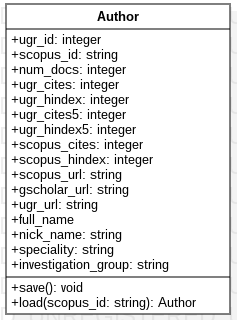
\includegraphics[width=0.4\linewidth]{imagenes/Author}
	\caption{Clase \textit{Author}}
\end{figure}

\newpage

\subsection{\textit{Abstract}}
\label{subsc:abstract}
La entidad \textit{Abstract} corresponde casi directamente con los datos obtenidos a través de la \acrshort{API} de Scopus, a excepción de:
\begin{itemize}
	\item Las referencias han sido limitadas a citas internas, es decir entre los artículos que están disponibles en la colección, con la idea de usar esta información en el proceso de búsqueda.
	\item Los autores, que únicamente aparecían listados con su \texttt{scopus\_id}, han sido enriquecidos con el nombre de los mismos así como el \texttt{ugr\_id} en caso de estar disponible este último (este identificador estará disponible si el autor es alguno de los que forman parte de la colección de autores).
\end{itemize}

\begin{figure}[h]
	
	\centering
	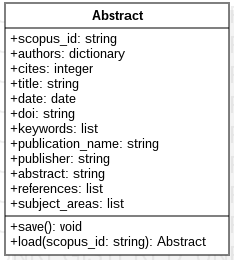
\includegraphics[width=0.4\linewidth]{imagenes/Abstract}
	\caption{Clase \textit{Abstract}}
\end{figure}

\newpage

\section{Arquitectura inicial del sistema}
\label{sc:arq_inicial}
La arquitectura del sistema planteado se basará en el modelo cliente/servidor con tres nodos:
\begin{itemize}
	\item \textbf{Servidor de \acrlong{BD}}: El cual almacenara la información correspondientes a autores y artículos como se ha modelado en el apartado previo.
	\item \textbf{Servidor de \acrshort{RI}}: Donde se llevará a cabo la búsqueda en sí, se servirá del servidor de \acrshort{BD} como almacenamiento de datos y atenderá las peticiones de búsqueda.
	\item \textbf{Cliente}: Parte del sistema que será visible para el usuario y que se encargará de recoger las peticiones de búsqueda, enviarlas al servidor de \acrshort{RI} y presentar los resultados devueltos por el mismo
\end{itemize}

\begin{figure}[ht]
	
	\centering
	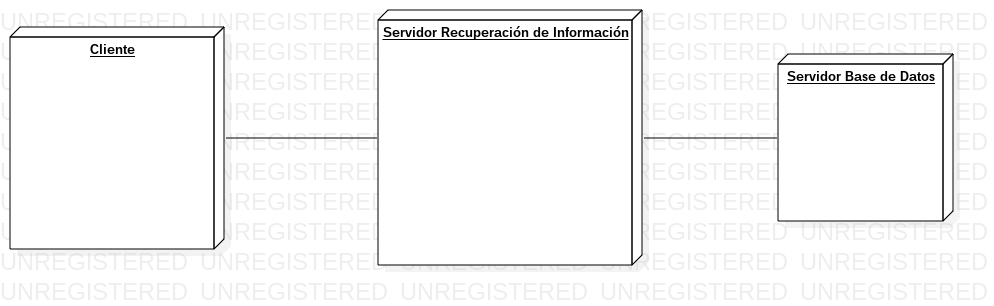
\includegraphics[width=\linewidth]{imagenes/initial_architecture}
	\caption{Diagrama de arquitectura inicial del sistema}

\end{figure}